\documentclass{article}
\usepackage{listings}
\documentclass[a4paper,10pt]{article}
\usepackage{siunitx}
\usepackage{spreadtab}
\usepackage{amsmath}
\usepackage[euler]{textgreek}
\usepackage{url}
\usepackage[siunitx]{circuitikz}
\usepackage{circuitikz}
\usepackage{siunitx}
\usepackage{placeins}
\usepackage{amssymb}
\usepackage{amsmath}

\input{./discussion/fwr_discussion_preamble.tex}
\usepackage[siunitx]{circuitikz}
\usepackage{circuitikz}
\usepackage{siunitx}
\usepackage{placeins}
\usepackage{amssymb}
\usepackage{amsmath}
\usepackage{csvsimple}

\usepackage[siunitx]{circuitikz}
\usepackage{circuitikz}
\usepackage{siunitx}
\usepackage{placeins}
\usepackage{amssymb}
\usepackage{amsmath}
\usepackage{csvsimple}

\begin{document}
	\begin{titlepage}
		\centering
		\Huge{Experiment 5} \\
		\huge{Transient Responses of Diodes and Rectifiers} \\
		\vspace{1cm}
		\large{EECS 170A - Lab Bench \#1} \\
		\large{\today} \\
		\vspace{1cm}
		\normalsize{Roman Parise (59611417)} \\
		\normalsize{Krishan Solanki (38154673)} \\
		\normalsize{Jason Wang (42873192)} \\
	\end{titlepage}
\section{Procedure}
\underline{Procedure}

For the second Electronics Lab, the objective is to solder RC circuits on a printed circuit board and then test the circuit as a Lowpass and Highpass Filter. To solder the resistor and capacitor, a soldering iron is used by melting metal onto the ends of the resistor and capacitor on a printed circuit board. After soldering, the output voltage in sine wave mode is measured at different frequencies using the oscilloscope. The Lowpass Filter has a function generator with internal resistance of (50\textOmega) which is in series with a 10k\textOmega resistor. The capacitor in this circuit is in parallel with the oscilloscope. The Highpass filter has a function generator with internal resistance of 50\textOmega  in series with a capacitor. The 10k\textOmega resistor is connected to the negative terminal of the function generator and is also in parallel with the oscilloscope. After taking the measurements, the transfer function ($H_{(s)} = \frac{V_o}{V_{in}$) for both filters are plotted as a function of frequency on a log-log scale. Lastly, the impulse response is measured by sending a pulse signal that is shorter than the RC time constant. The measured responses are then compared to the theoretical responses. \\
\\
\underline{LowPass Filter}
\\
\centerline{ $ H_{(s)} = \frac{V_o}{V_{in}} = \frac{Z_c}{Z_r + Z_c} $ }
\centerline{ $ Z_r = R, Z_c = \frac{1}{sc} $}
\centerline{ $ H_{(s)} = \frac{V_o}{V_{in}} = \frac{\frac{1}{sc}}{R + \frac{1}{sc}} $ }
\begin{equation}
\label{eq:LowPassFunction}
\centerline{ $ H_{(s)} = \frac{V_o}{V_{in}} = \frac{1}{sRC + 1} $ }
\end{equation}
\\
\underline{HighPass Filter}
\\
\centerline{ $ H_{(s)} = \frac{V_o}{V_{in}} = \frac{Z_r}{Z_r + Z_c} $ }
\centerline{ $ Z_r = R, Z_c = \frac{1}{sc} $}
\centerline{ $ H_{(s)} = \frac{V_o}{V_{in}} = \frac{R}{R + \frac{1}{sc}} $ }
\begin{equation}
\label{eq:HighPassFunction}
\centerline{ $ H_{(s)} = \frac{V_o}{V_{in}} = \frac{sRC}{sRC + 1} $ }
\end{equation}





\section{Results and Analysis}
\subsection{Transient Response of Diodes}
\subsubsection{pn-Junction Diode}
The following circuit is used to analyze the transient responses or switching behaviors of pn-junction diodes, Schottky diodes, and switching diodes:
\FloatBarrier
\begin{figure}[h!]
	\centering
	\caption{Circuit Schematic for Diode Transient Response Analysis}
	\label{fig:dtr}
\begin{circuitikz} \draw
	( 0 , 4 ) to [ sqV , v<=$20Vpp$ ] ( 0 , 0 )
	( 0 , 4 ) to [ empty diode ] ( 4 , 4 )
	( 4 , 4 ) to [ R = 300 <\ohm> ] ( 4 , 0 ) -- ( 0 , 0 ) ;
\end{circuitikz}
\end{figure}
\FloatBarrier

The empty diode represents the different types of diodes analyzed and a square source with positive edge at $10V$ and negative edge at $-10V$ is used ($20Vpp$) with a frequency of $10 kHz$. The positive and negative edges of the square source applies a forward and reverse bias respectively on the tested diodes. Because of the sharp transition from the positive to negative edge of the source, switching behavior is to be observed in the diode circuit.

When forward bias is applied to a pn-junction diode, an electric field is generated across the diode from the p-region to the n-region. This causes excess holes from the p-region to migrate across the depletion region to the n-region and excess electrons from the n-region to migrate to the p-region. The migrated charge carriers are the excess minority charge carriers of the quasi-neutral regions that they migrated to and are effectively "stored" in the new regions that they reside in. The current through the diode after an adequately long duration of time reaches a constant current, $I_{F}$, at steady state.

When the square source wave undergoes the sharp transition from its positive to negative edge, a reverse bias is abruptly applied to the pn-junction diode and the electric field across the pn-junction diode is immediately reversed. The reversal in polarity of the electric field causes the excess minority carriers to flow out of their respective quasi-neutral regions and recombine with donor and acceptor ions on the other side. This movement of carriers causes a reverse current, $I_{R}$, that is much greater in magnitude than the reverse saturation current, $I_{S}$ (ideally, $I_{S}$ is approximately $0.1I_{R}$). The withdrawal of the stored excess minority carriers across the depletion region causes the reverse current to be close to constant for a duration called the storage time, $t_{s}$. After that period of time, the reverse current then decays to the reverse saturation current.

The storage time, $t_{s}$ is ideally represented in the following equation:
\begin{equation}
\label{eq:diode_t_s}
erf(\sqrt{\frac{t_{s}}{\tau_{p}}}) = \frac{1}{1+\frac{I_{R}}{I_{F}}}
\end{equation}
where $\tau_{p}$ is minority carrier lifetime and $erf(\xi)$ is the error function defined to be:
\begin{equation}
\label{eq:erf}
erf(\xi) = \frac{2}{\sqrt{\pi}}\int_{0}^{\xi}e^{-x^{2}}dx
\end{equation}

Effectively, because of the interactions of excess charge carriers within the pn-junction diode, a delay is to be observed in the rectification of the reverse signal and the current waveform of the pn-junction diode should have the following shape:
\FloatBarrier
\begin{figure}[h!]
	\centering
	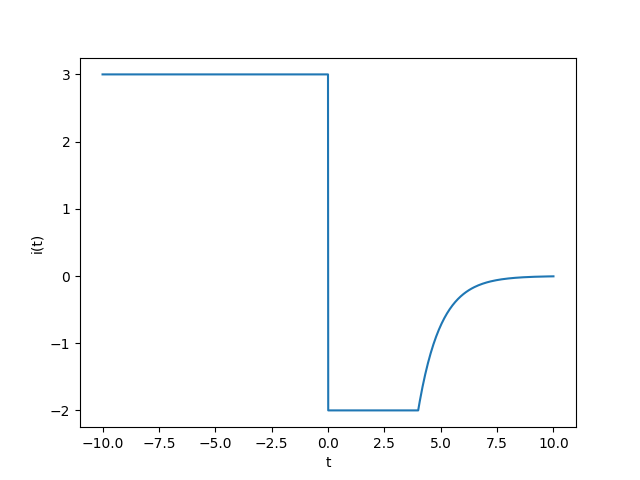
\includegraphics[scale=0.75]{./images/diode_current.PNG}
	\caption{pn-Junction Diode Expected Current Waveform}
	\label{fig:diode_current}
\end{figure}
\FloatBarrier
Also, the voltage waveform of the diode should also have an observable delay in switching polarity and the waveform should look like the following:
\FloatBarrier
\begin{figure}[h!]
	\centering
	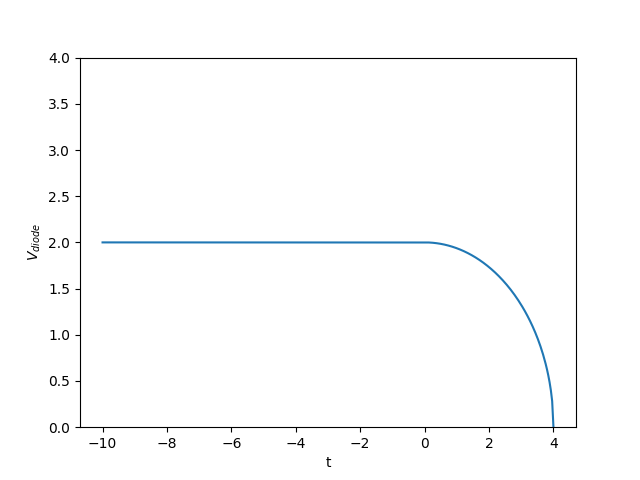
\includegraphics[scale=0.75]{./images/diode_voltage.PNG}
	\caption{pn-Junction Diode Expected Current Waveform}
	\label{fig:diode_voltage}
\end{figure}
\FloatBarrier
*Note that for both Figures (\ref{fig:diode_current}) and (\ref{fig:diode_voltage}), the source voltage switches at $t=0$.

In the observation of the pn-junction diode, the following waveform is observed for the voltage across the $300\Omega$ resistor where the top wave is the voltage across the resistor and the bottom wave is the source voltage:
\FloatBarrier
\begin{figure}[h!]
	\centering
	\includegraphics[scale=0.25]{./images/pn_junction_diode_transient_response.jpg}
	\caption{pn-Junction Diode Observed Voltage Across Resistor}
	\label{fig:pn_diode_v_r}
\end{figure}
\FloatBarrier
The following waveform is then observed for the voltage across the pn-junction diode:
\FloatBarrier
\begin{figure}[h!]
	\centering
	\includegraphics[scale=0.25]{./images/pn_junction_diode_v_diode.jpg}
	\caption{pn-Junction Diode Observed Voltage Across Diode}
	\label{fig:pn_diode_v_d}
\end{figure}
\FloatBarrier
The forward and reverse voltages of the pn-junction diode are then measured to be the following:
\begin{equation}
\label{eq:pn_measured_vfr}
V_{F}=8.375V,V_{R}=-9.8125V
\end{equation}
The current through the diode and the voltage across the resistor have a simple Ohmic relationship, so the forward and reverse currents can be found by doing the calculation below:
\begin{equation}
\label{eq:ifr_vs_vfr}
I_{F/R}=\frac{V_{F/R}}{R_L}=\frac{V_{F/R}}{300\Omega}
\end{equation}
The following results for forward and reverse currents are then calculated:
\begin{equation}
\label{eq:pn_measured_ifr}
I_{F}=27.91mA,I_{R}=-32.71mA
\end{equation}

By employing KCL, the following equation can be utilized to find the theoretical value for $I_F$:
\begin{equation}
\label{eq:if_theory}
I_F = \frac{V_P-V_{on}}{R_L}
\end{equation}
and this equation for the theoretical value of $I_R$
\begin{equation}
\label{eq:ir_theory}
I_F = \frac{V_N+V_{on}}{R_L}
\end{equation}
By substituting the values $V_P = 10V$, $V_N = -10V$, and $V_{on} = 0.7V$, the following theoretical values are calculated:
\begin{equation}
\label{eq:pn_theoretical_ifr}
I_{F}=31mA,I_{R}=-31mA
\end{equation}
The percent errors for $I_F$ and $I_R$ respectively are $-10.0\%$ and $-5.5\%$.
\FloatBarrier
\begin{table}[h!]
	\centering
	\caption{Measured vs. Theoretical Forward and Reverse Currents for pn-Junction Diode}
	\label{tab:pn_ifr}
	\csvautotabular{./tables/pn_ifr.csv}
\end{table}
\FloatBarrier

Zooming in to the region in the which the delay occurs allows for the storage time to be more clearly observed and measured:
\FloatBarrier
\begin{figure}[h!]
	\centering
	\includegraphics[scale=0.25]{./images/pn_junction_storage_time_v_resistor.jpg}
	\caption{pn-Junction Diode Observed Storage Time}
	\label{fig:pn_diode_t_s}
\end{figure}
\FloatBarrier
The storage time of the pn-junction diode measured from the oscilloscope is the following:
\begin{equation}
\label{eq:pn_measured_t_s}
t_{s}=2.97\mu s
\end{equation}
After measuring the storage time of three other diodes, the following values for storage times are found:
\FloatBarrier
\begin{table}[h!]
	\centering
	\caption{Measured Storage Times of Various pn-Junction Diodes}
	\label{tab:pn_ts}
	\csvautotabular{./tables/pn_ts.csv}
\end{table}
\FloatBarrier
By observation, the first storage time measurement seems to be an outlier.

\subsubsection{Schottky Diode}
For the Schottky diode, the following waveform for voltage across the resistor is observed (top waveform is source voltage and bottom waveform is the voltage across the resistor):
\FloatBarrier
\begin{figure}[h!]
	\centering
	\includegraphics[scale=0.25]{./images/schottky_diode_input_output_waveforms.jpg}
	\caption{Schottky Diode Observed Voltage Across Resistor}
	\label{fig:schottky_vr}
\end{figure}
\FloatBarrier
The following would then be the observed waveform for voltage across the diode:
\FloatBarrier
\begin{figure}[h!]
	\centering
	\includegraphics[scale=0.25]{./images/schottky_diode_v_diode.jpg}
	\caption{Schottky Diode Observed Voltage Across Diode}
	\label{fig:schottky_vd}
\end{figure}
\FloatBarrier
In both oscilloscope plots (Figures (\ref{fig:schottky_vr}) and (\ref{fig:schottky_vd})), there is no observable delay in the rectification of the source signal for the Schottky diode. This is expected behavior due to the physical features of the Schottky diode. The Schottky diode differs fundamentally from a pn-junction diode in that it utilizes metal-semiconductor junction where the semiconductor is n-type(M-S junction). A depletion region created by the M-S junction is negligible compared to that of a pn-junction (\ref{ref:schottky}). Also, while pn-junction diodes rely on both electrons and holes to carry electric current, Schottky diodes only utilize electrons (\ref{ref:schottky}). Because of this physical property, there are no excess minority carriers that accumulate at quasi-neutral regions, thus no storage time should be observed and switching time is near instantaneous.
\subsection{Full-Wave Bridge Rectifier}
\FloatBarrier

\begin{figure}[h!]
\centering
\caption{Full-Wave Bridge Rectifier Circuit}
\label{fig:fwr}
\begin{circuitikz}
	\draw
	( 0 , 4 ) to [ sV , v<=$20Vpp$ ] ( 0 , 0 )
	( 0 , 4 ) -- ( 4 , 4 ) to [ empty diode ] ( 6 , 2 )
	( 2 , 2 ) to [ empty diode ] ( 4 , 4 )
	( 2 , 2 ) to [ empty diode ] ( 4 , 0 )
	( 4 , 0 ) to [ empty diode ] ( 6 , 2 )
	( 4 , 0 ) -- ( 0 , 0 )
	( 2 , 2 ) to [ R = 300 <\ohm> ] ( 6 , 2 )
	( 2 , 2 ) node[label={ [font=\normalsize] above : $-$ } ] { }
	( 6 , 2 ) node[label={ [font=\normalsize] above : $+$ } ] { }
	;
\end{circuitikz}
\end{figure}

\FloatBarrier

Figure (\ref{fig:fwr}) displays a full-wave bridge rectifier circuit. The circuit's specification requires that it take an input sinusoidal signal and produce an output voltage that is the absolute value of that signal with the least amount of error possible. The output voltage is measured over the resistor, which shall be referred to as $R$. In reality, this ideal is not reached. The experiment demonstrates the degree to which the specification is satisfied.
The full-wave bridge rectifier circuit takes advantage of the fact that diodes essentially act as broken circuits when the applied voltage is less than its threshold voltage and act as short circuits when the applied voltage exceeds its threshold voltage. This is a simplification of the Shockley diode model:

\begin{equation}
	\label{eq:shockley_diode}
	I_{diode}( V_{applied} ) = I_0 ( e^{ \frac{qV_{applied}}{k_B T} } - 1 )
\end{equation}

In equation (\ref{eq:shockley_diode}), $I_0$ is the reverse saturation current, $q$ is the elementary charge, $k_B$ is Boltzmann's constant, and $T$ is temperature. A more ideal model treats the diode as the perfect switch described above, namely that the diode acts as a broken circuit unless $V_{applied}$ exceeds its threshold voltage, assumed to be about 0.7\si{\volt} and referred to as $V_{Th}$. Figure (\ref{fig:ideal_vs_shock}) below compares these two models in a graph. The graph demonstrates that this more idealized model accurately characterizes the behavior of the diode. It shall be used instead to describe the diode's characteristics.

\FloatBarrier

\begin{figure}[h!]
	\centering
	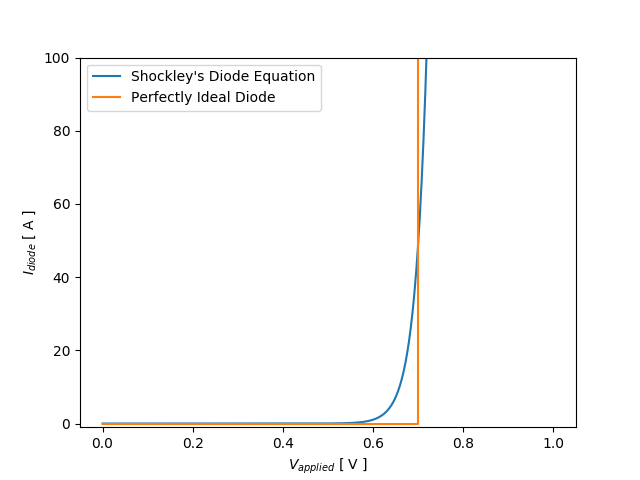
\includegraphics[scale=0.75]{../images/ideal_diode.PNG}
	\caption{Shockley Diode Model vs. Perfectly Ideal Diode}
	\label{fig:ideal_vs_shock}
\end{figure}

\FloatBarrier

{\footnotesize $I_0$ is set to 0.1\si{\nano\ampere}. Temperature is assumed to be 300\si{\kelvin}. Threshold voltage of perfectly ideal model is assumed to be 0.7\si{\volt}. }

\FloatBarrier

A diode is said to be enabled when the applied source voltage, which shall be called $V_{A}$, meets or exceeds its threshold voltage. Enabled diodes are drawn in green. Two cases are to be considered: when $V_{A} > 2V_{Th}$ and when $V_{A} < 2V_{Th}$. $2V_{Th}$ must be used since the voltage must enabled two diodes in series as seen in the figures below. Note that $|V_{A}| < 2V_{Th}$ is trivial since no voltage drops over the load resistor $R$.

When $V_{A} > 2V_{Th}$, the diodes in figure (\ref{fig:v_app_high}) are enabled. The voltage measured over the resistor is clearly positive due to the direction of positive current flow. The positive current flow direction is indicated by an arrow.

\FloatBarrier

\begin{figure}[h!]
\centering
\caption{Full-Wave Rectifier when $V_{A} > 2V_{Th}$}
\label{fig:v_app_high}
\begin{circuitikz}
	\draw
	( 0 , 4 ) to [ sV , v<=$20Vpp$ ] ( 0 , 0 )
	( 0 , 4 ) -- ( 4 , 4 ) to [ empty diode , color = green ] ( 6 , 2 )
	( 2 , 2 ) to [ empty diode ] ( 4 , 4 )
	( 2 , 2 ) to [ empty diode , color = green ] ( 4 , 0 )
	( 4 , 0 ) to [ empty diode ] ( 6 , 2 )
	( 4 , 0 ) -- ( 0 , 0 )
	( 2 , 2 ) to [ R = 300 <\ohm> , i<_=$I$ ] ( 6 , 2 )
	( 2 , 2 ) node[label={ [font=\normalsize] above : $-$ } ] { }
	( 6 , 2 ) node[label={ [font=\normalsize] above : $+$ } ] { }
	;
\end{circuitikz}
\end{figure}

\FloatBarrier

Figure (\ref{fig:v_app_low}) demonstrates the case when $V_{A} < 2V_{Th}$. Again, the output voltage taken over the resistor is positive due to the direction of positive current flow.

\FloatBarrier

\begin{figure}[h!]
\centering
\caption{Full-Wave Rectifier when $V_{A} < 2V_{Th}$}
\label{fig:v_app_low}
\begin{circuitikz}
	\draw
	( 0 , 4 ) to [ sV , v<=$20Vpp$ ] ( 0 , 0 )
	( 0 , 4 ) -- ( 4 , 4 ) to [ empty diode ] ( 6 , 2 )
	( 2 , 2 ) to [ empty diode , color = green ] ( 4 , 4 )
	( 2 , 2 ) to [ empty diode ] ( 4 , 0 )
	( 4 , 0 ) to [ empty diode , color = green ] ( 6 , 2 )
	( 4 , 0 ) -- ( 0 , 0 )
	( 2 , 2 ) to [ R = 300 <\ohm> , i<_=$I$ ] ( 6 , 2 )
	( 2 , 2 ) node[label={ [font=\normalsize] above : $-$ } ] { }
	( 6 , 2 ) node[label={ [font=\normalsize] above : $+$ } ] { }
	;
\end{circuitikz}
\end{figure}

\FloatBarrier

A more quantitative description of this behavior can be obtained. In the $V_{A} > 2V_{Th}$ case, Kirchhoff's voltage law may be applied:

\FloatBarrier

\begin{figure}[h!]
\centering
\caption{Kirchhoff's Voltage Law for $V_{A} > 2V_{Th}$}
\label{fig:kvl_app_high}
\begin{circuitikz}
	\draw
	( 0 , 4 ) to [ sV , v<=$20Vpp$ ] ( 0 , 0 )
	( 0 , 4 ) -- ( 4 , 4 ) to [ empty diode , color = green ] ( 6 , 2 )
	( 2 , 2 ) to [ empty diode , color = green ] ( 4 , 0 )
	( 4 , 0 ) -- ( 0 , 0 )
	( 2 , 2 ) to [ R = 300 <\ohm> , i<_=$I$ ] ( 6 , 2 )
	( 2 , 2 ) node[label={ [font=\normalsize] above : $-$ } ] { }
	( 6 , 2 ) node[label={ [font=\normalsize] above : $+$ } ] { }
	( 1.5 , 1 ) node[scale=3]{$\circlearrowright$}
	;
\end{circuitikz}
\end{figure}

\FloatBarrier

\begin{equation}
	\label{eq:kvl_va_gt_2vth}
	+V_{A} - V_{Th} - V_{out} - V_{Th} = 0 \rightarrow V_{out} = V_{A} - 2V_{Th}
\end{equation}

The same method can be applied to the $V_{A} < 2V_{Th}$ case.

\FloatBarrier

\begin{figure}[h!]
\centering
\caption{Kirchhoff's Voltage Law for $V_{A} > 2V_{Th}$}
\label{fig:kvl_app_low}
\begin{circuitikz}
	\draw
	( 0 , 4 ) to [ sV , v<=$20Vpp$ ] ( 0 , 0 )
	( 0 , 4 ) -- ( 4 , 4 )
	( 2 , 2 ) to [ empty diode , color = green ] ( 4 , 4 )
	( 4 , 0 ) to [ empty diode , color = green ] ( 6 , 2 )
	( 4 , 0 ) -- ( 0 , 0 )
	( 2 , 2 ) to [ R = 300 <\ohm> , i<_=$I$ ] ( 6 , 2 )
	( 2 , 2 ) node[label={ [font=\normalsize] above : $-$ } ] { }
	( 6 , 2 ) node[label={ [font=\normalsize] above : $+$ } ] { }
	( 1.5 , 1 ) node[scale=3]{$\circlearrowright$}
	;
\end{circuitikz}
\end{figure}

\FloatBarrier

\begin{equation}
	\label{eq:kvl_va_lt_2vth}
	+V_{A} + V_{Th} + V_{out} + V_{Th} = 0 \rightarrow V_{out} = - V_{A} - 2V_{Th}
\end{equation}

These behaviors can be generalized in the following result for the output voltage of the full-wave rectifier circuit in figure (\ref{fig:fwr}):

\begin{equation}
	\label{eq:fwr_eq}
	V_{out}(V_{A}) =
	\begin{cases}
		|V_{A}| - 2V_{Th} , & |V_{A}| > 2V_{Th} \\
		0 , & \text{otherwise}
	\end{cases}
\end{equation}

A plot of the expected output voltage against the input voltage is shown in figure (\ref{fig:expected_out_vs_in_fwr}):

\FloatBarrier

\begin{figure}[h!]
	\centering
	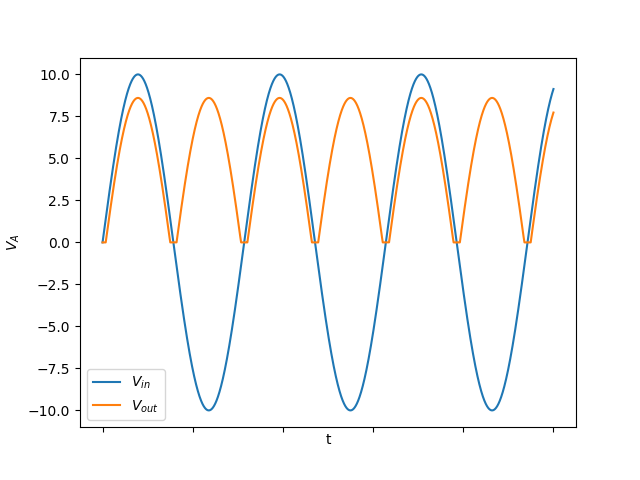
\includegraphics[scale=0.75]{../images/full_wave_rect.PNG}
	\caption{Full-Wave Bridge Rectifier Expected Result}
	\label{fig:expected_out_vs_in_fwr}
\end{figure}

\FloatBarrier


\section{Discussion}
\subsection{Transient Response of Diodes}
Both the pn-junction diode and Schottky diode yielded waveforms that agree well with theory. In analyzing the two types of diodes, the advantages and disadvantages of each are made clear. The Schottky diode is observed to have a nonexistent storage time whereas the pn-junction diode is observed to have a storage time of approximately $4\mu s$. The very apparent delay in rectification from the storage time of the pn-junction diode makes that type of diode not suited for high frequency applications. The Schottky diode, however, is very commonly used in high frequency applications like RF. What is not shown in this experiment is that Schottky diodes have significantly lower reverse breakdown voltages than pn-junction diodes  (\ref{ref:schottky2}), therefore Schottky diodes may not be suitable for high voltage environments. 
It should also be noted that the diode's 10\% error or so in Table (1) is likely a result of nonidealities in the manufacturing process of both the diode and the resistor. The resistor used in the measurement likely deviates from the $300\Omega$ value, and the diode has some internal resistance as well. Moreover, the diode's properties, such as $V_{on}$ in equations (5) and (6) are also subject to variations in the manufacturing process, such as in doping concentrations. The important part of the experiment is the shape of the waveform in figure (4). Better characterization of the properties of the resistor and the diode are required for more accurate results.

\subsection{Full-Wave Bridge Rectifier}
The full-wave bridge rectifier results align quite well with theory. However, the peak measurement does have slightly more error than the trough measurement. These errors are a result of either an asymmetry in the source voltage or an asymmetry in the threshold voltages of the diodes. The former is not possible to prove due to the fact that the source voltage is not probed in the experiment. However, if the sinusoidal source voltage's peak is higher than the reported value on the power supply, this would explain why the measured voltage for the output voltage's peak is higher than expected. Furthermore, the diodes may differ in threshold voltage. Differences in threshold voltage are a result of either temperature, material, or doping variations:

\begin{align*}
	\label{eq:vbi}
	V_{bi} = \frac{k_BT}{q} ln( \frac{N_AN_D}{(n_{i}(T))^2} )
\end{align*}

Temperature is likely not the cause since the temperature in the room in which the experiment is conducted is essentially uniform, which would not explain the asymmetry in the measurements. A better explanation is that the doping concentrations vary slightly from diode to diode due to slight nonidealities in the manufacturing process. So, the diodes along the enabled path when the source voltage is positive could have slightly lower threshold voltages than the diodes along the other path.

\section{Appendix}
The following script is used to generate the theoretical pn-junction diode current plot in figure (\ref{fig:diode_current}):
\lstinputlisting[breaklines]{./scripts/diode_current.py}
The following script is used to generate the theoretical pn-junction diode voltage plot in figure (\ref{fig:diode_voltage}):
\lstinputlisting[breaklines]{./scripts/diode_voltage.py}
The following script is used to generate the theoretical full-wave recitifer plot in figure (\ref{fig:expected_out_vs_in_fwr}):
\lstinputlisting[breaklines]{./scripts/full_wave_rect.py}
The following script is used to generate tables (\ref{tab:peak_n_trough}) and (\ref{tab:theory_vs_practice}):
\lstinputlisting[breaklines]{./scripts/fwr_data.py}
Lastly, this script is used to generate figure (\ref{fig:ideal_vs_shock}):
\lstinputlisting[breaklines]{./scripts/gen_ideal_diode.py}
\section{References}
\begin{enumerate}
	\item \label{ref:schottky} \url{https://tex.stackexchange.com/questions/236359/making-a-list-of-websites}
	\item \label{ref:schottky2} \url{http://www.radio-electronics.com/info/data/semicond/schottky_diode/schottky_barrier_diode.php}
\end{enumerate}
\end{document}
